\section*{6.3 Bad Parallelization of AlphaBeta}

\subsection*{1. Comparison of total number of evaluations of minimax and abid}


\begin{center}
  \begin{tabular}{|r|r|r|}
    \hline
    Setting & MiniMax & AlphaBeta \\ \hline
    midgame1, depth2 & 5,199 & 4,866 \\ \hline
    midgame1, depth3 & 120,718 & 49,198    \\ \hline
    midgame1, depth4 & 2,485,542 & 916,465    \\ \hline
    midgame1, depth5 & 15,018,100 & 4,120,198    \\ \hline
    midgame2, depth2 & 4,358 & 4,577 \\ \hline
    midgame2, depth3 & 97,908 & 43,335    \\ \hline
    midgame2, depth4 & 1,519,234 & 531,259   \\ \hline
    midgame2, depth5 & 4,411,737 & 2,067,878    \\ \hline
    endgame, depth2 & 1,796 & 3,602 \\ \hline
    endgame, depth3 & 17,823 & 9,801    \\ \hline
    endgame, depth4 & 23,266 & 17,643   \\ \hline
    endgame, depth5 & 1,520,313 & 402,920    \\ \hline
  \end{tabular}
\end{center}

There is two things one can easily spot: For small depths, alphabeta might actually need more evaluations than minimax. This assumption, however, is not correct, as a pure alphabeta cannot evaluate more moves than minimax. The overhead in this case is caused by optimizations applied to alphabeta, mainly iterative deepening, but also by first trying to initialize the alphabeta window with reasonable values, as there is not a lot to optimize for such flat trees. Second, you can cleary spot, that those optimizations as well as the general alphabeta approach do a good job when it comes to reducing the size of search trees with huge depth. 

\subsection*{2. Naive Parallelization, Overhead}
We decided to decompose the moves at the topmost layer in the alphabeta method and leave the searchbestmove method untouched, as it does things we cannot really parallelize (to parallelize iterative deepening is cleary not advantageous, because the idea is to reuse the results from the calculation for depth-1 when calculating the values for depth, and parallelizing the alphabeta-calls with different windows is not smart, because we assume that the reasonable values are actually reasonable, and you can see from the fact that there is not a lot of calls of alphabeta with the same maxdepth that they are.) We used a master/slave(worker) approach, so that the root process distributes one move at a time to a process, and also sent the corresponding alphabeta window to each process with the particular move. We did this, because the window might have updated and we want to allow processes to prune quickly if they can.

\begin{center}
  \begin{tabular}{|r|r|r|r|r|r|}
    \hline
    Setting & AlphaBeta & Overhead 2 workers & 4 processes (3w) & 6p (5w)& 8p (7w)\\ \hline
    midgame1, depth5 & 4,120,198 & 18.8\% & 19.5\% & 24.8\% & 22.6\% \\ \hline
    midgame2, depth5 & 2,067,878 & 6.6\% & 29.6\% & 44.7\% & 59.2\% \\ \hline
    endgame, depth5 & 402,920 & 162\% & 300.1\% & 631\% & 644.5\%  \\ \hline
  \end{tabular}
\end{center}

The reason for the search overhead is easy to understand. When the sequential version works through the tree, it already knows the value of node1 at any depth while evaluating node2 (assuming that node 2 is on the righthand side of node1, i.e. we are enumerating from left to right) at the very same depth and therefore can easily decide whether to prune or not. In a parallel version, there is n nodes (with n being the number of workers) which are being evaluated with the same alphabeta values, because they are running concurrently. Those processes therefore have older values to use when deciding whether to prune or not, and have to do more evaluations. In particular cases, where predicting the alphabeta window while using iterative deepening fails, you will have a large amount of overhead as there are going to be depthsearches with a broad window and high depth. Where a sequential algorithm only has to traverse the first node with the broad window, the parallel version must traverse n (with n again being the number of workers) nodes with the broad window (or, in our case n+1, as the masterprocess sends out a new task before reading the values returned by the worker), resulting in plenty of overhead. Exactly this issue happens in position-endgame, leading to the incredible amount of overhead
The values are only computed for more than one worker, but due to the master/worker approach, you could actually expect overhead for one worker as well, because the master process already sends out a new task before processing the data returned by the worker.

\subsection*{Speedup}

In general, the result is better than expected, mainly because the iterative deepening and adaptive alphabeta-window do a good job narrowing down search windows for deapthsearches with high levels. However, you can see the devastating effects the mispredicted alphabeta-window for position-endgame has.

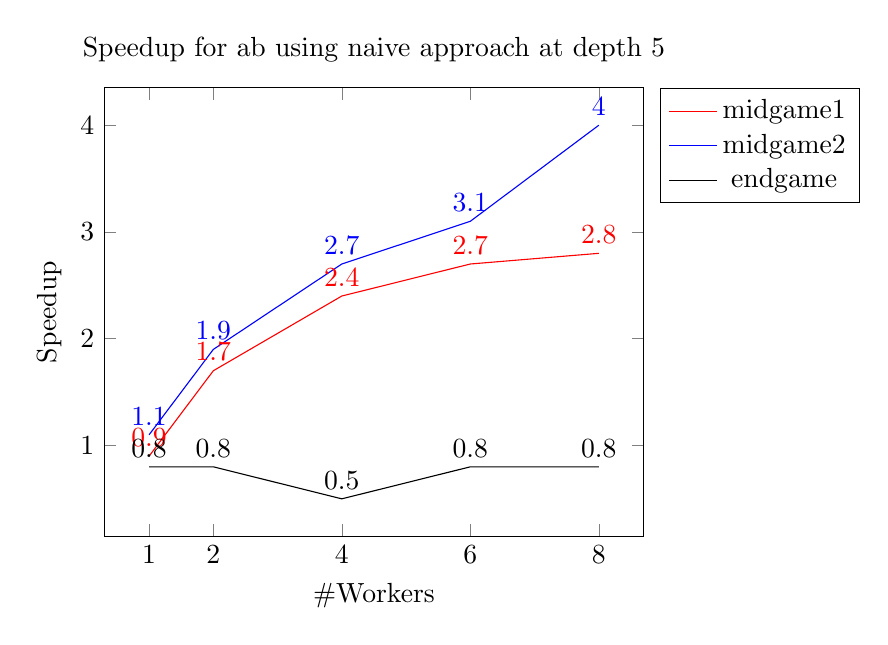
\begin{tikzpicture}
  \begin{axis}[
      legend style={cells={align=left}},
      xtick={1, 2, 4, 6, 8},
      xlabel=\#Workers,
      ylabel=Speedup,
      title=Speedup for ab using naive approach at depth 5,
      legend pos = outer north east,
      nodes near coords,
      scaled ticks = false,
      y tick label style={
        /pgf/number format/.cd,
	fixed,
        fixed zerofill,
	precision=0,
        /tikz/.cd
      },
      no markers]
     \addplot[color=red] coordinates {
       (1,0.9)
       (2,1.7)
       (4,2.4)
       (6,2.7)
       (8,2.8)
     };
     \addplot[color=blue] coordinates {
       (1,1.1)
       (2,1.9)
       (4,2.7)
       (6,3.1)
       (8,4.0)
     };
     \addplot[color=black] coordinates {
       (1,0.8)
       (2,0.8)
       (4,0.5)
       (6,0.8)
       (8,0.8)
     };
     \legend{midgame1, midgame2, endgame}
  \end{axis}
  
\end{tikzpicture}
